\documentclass{standalone}
\usepackage{tikz}
\usetikzlibrary{arrows.meta}

\begin{document}
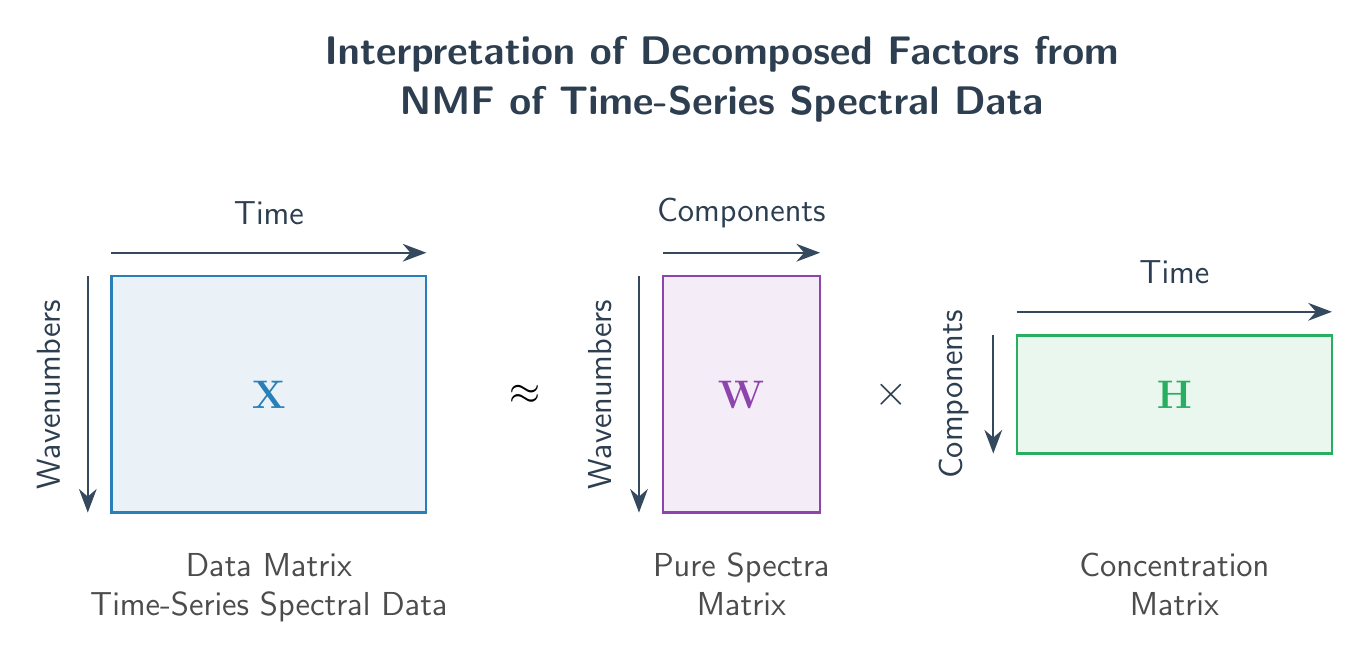
\begin{tikzpicture}[
    every node/.style={font=\large\sffamily},
    matrix label/.style={font=\Large\bfseries\sffamily, text=black!80},
    info/.style={font=\large\sffamily, text=black!70, align=center}
]
\definecolor{xmatrix}{RGB}{41,128,185}    % Blue
\definecolor{wmatrix}{RGB}{142,68,173}    % Purple
\definecolor{hmatrix}{RGB}{39,174,96}     % Green
\definecolor{arrowcolor}{RGB}{52,73,94}   % Dark blue-grey
\definecolor{labelcolor}{RGB}{44,62,80}   % Darker blue-grey

% Calculate the horizontal center of the diagram
\path (0,0) -- (15.5,0) node[coordinate, pos=0.5] (center) {};

% Title at the top with two lines and centered
\node[font=\Large\bfseries\sffamily, text=labelcolor, align=center, anchor=center] at (center |- 0,5.5)
{Interpretation of Decomposed Factors from\\NMF of Time-Series Spectral Data};

\draw[thick, xmatrix, fill=xmatrix!10] (0,0) rectangle (4,3);
\node[matrix label, text=xmatrix] at (2,1.5) {$\mathbf{X}$};
\node[text=labelcolor] at (2, 3.8) {Time};
\draw[-{Stealth[length=3mm]}, thick, arrowcolor] (0,3.3) -- (4,3.3);
\node[rotate=90, anchor=center, text=labelcolor] at (-0.8,1.5) {Wavenumbers};
\draw[-{Stealth[length=3mm]}, thick, arrowcolor] (-0.3,3) -- (-0.3,0);
\node[info, below] at (2,-0.4) {Data Matrix\\Time-Series Spectral Data};

\node[scale=1.2] at (5.25,1.5) {$\approx$};

\draw[thick, wmatrix, fill=wmatrix!10] (7,0) rectangle (9,3);
\node[matrix label, text=wmatrix] at (8,1.5) {$\mathbf{W}$};
\node[text=labelcolor] at (8,3.8) {Components};
\draw[-{Stealth[length=3mm]}, thick, arrowcolor] (7,3.3) -- (9,3.3);
\node[rotate=90, anchor=center, text=labelcolor] at (6.2,1.5) {Wavenumbers};
\draw[-{Stealth[length=3mm]}, thick, arrowcolor] (6.7,3) -- (6.7,0);
\node[info, below] at (8,-0.4) {Pure Spectra\\Matrix};

\node[scale=1.3] at (9.9,1.5) {\textcolor{labelcolor}{$\times$}};

\draw[thick, hmatrix, fill=hmatrix!10] (11.5,0.75) rectangle (15.5,2.25);
\node[matrix label, text=hmatrix] at (13.5,1.5) {$\mathbf{H}$};
\node[text=labelcolor] at (13.5,3.05) {Time};
\draw[-{Stealth[length=3mm]}, thick, arrowcolor] (11.5,2.55) -- (15.5,2.55);
\node[rotate=90, anchor=center, text=labelcolor] at (10.7,1.5) {Components};
\draw[-{Stealth[length=3mm]}, thick, arrowcolor] (11.2,2.25) -- (11.2,0.75);
\node[info, below] at (13.5,-0.4) {Concentration\\Matrix};

\end{tikzpicture}
\end{document}